\documentclass{article} % For LaTeX2e
\usepackage{nips15submit_e,times}
\usepackage{hyperref}
\usepackage{url}
\usepackage{graphicx}
\usepackage{array}
\usepackage{afterpage}
%\documentstyle[nips14submit_09,times,art10]{article} % For LaTeX 2.09

\title{EEG curiosities -- follow-up II}

\author{
Manuel Nickel
\\
%Technische Universit\"at M\"unchen\\
%Pittsburgh, PA 15213 \\
\texttt{manuel.nickel@tum.de} \\
\And
Dominik Irimi \\
%Affiliation \\
%Address \\
\texttt{dominik.irimi@gmail.com} \\
\AND
Christoph Dehner \\
%Affiliation \\
%Address \\
\texttt{dehner@in.tum.de} \\
\And
Roman C.~Podolski \\
%Affiliation \\
%Address \\
\texttt{roman.podolski@tum.de} \\
\And
Philipp Bergmann \\
%Affiliation \\
%Address \\
\texttt{philipp.bergmann@tum.de} \\
}

% The \author macro works with any number of authors. There are two commands
% used to separate the names and addresses of multiple authors: \And and \AND.
%
% Using \And between authors leaves it to \LaTeX{} to determine where to break
% the lines. Using \AND forces a linebreak at that point. So, if \LaTeX{}
% puts 3 of 4 authors names on the first line, and the last on the second
% line, try using \AND instead of \And before the third author name.

\newcommand{\fix}{\marginpar{FIX}}
\newcommand{\new}{\marginpar{NEW}}

\nipsfinalcopy % Uncomment for camera-ready version

\begin{document}


\maketitle

\begin{abstract}
Yet again, test runs were performed, this time normalizing the datasets trial-wise.
\end{abstract}

\section{Normalizing trial-wise}
Trial-wise normalization of the EEG data was implemented. In order to check its correct function, t-SNE runs as well as neural net runs were once again performed on the artificial reference datasets. In particular, \verb|sp_var| was used. In this, all data points were Gaussian with the same variance. But for each trial a mean with a different offset was used. Thus, this ideally shows if the normalization is working correctly. 

For testing purposes, t-SNE and the neural net were applied on the data points of five trials in \verb|sp_var|. Figure \ref{fig:sp_var_nT} shows the \verb|sp_var| data plotted after normalization with respect to the entire set -- which will be from now on refered to as unit-normalization. The inherent structure thus is not changed and each trial is shown well separated from the others. Figure \ref{fig:sp_var_nF} on the other hand shows the result for running t-SNE on \verb|sp_var| normalized trial-wise. As expected, each trial's mean is shifted to $0$ and thus all trials are grouped into one single big cluster. The normalization procedure thus appears to be working fine. The neural net outputs expected results, too. For the unit-normalized dataset an error rate of $0.00\%$ was achieved. In the trial-wise normalized case the error would just be as bad as $97.11\%$. Figure \ref{fig:sp_var_double} shows the error curves for the two normalization methods. The dotted line represents unit-normalization, while the continuous line stands for trial-wise normalization. The neural net thus seems to be set up properly, as well.

\begin{figure}
	\centering
	\begin{minipage}{0.5\textwidth}
		\centering
		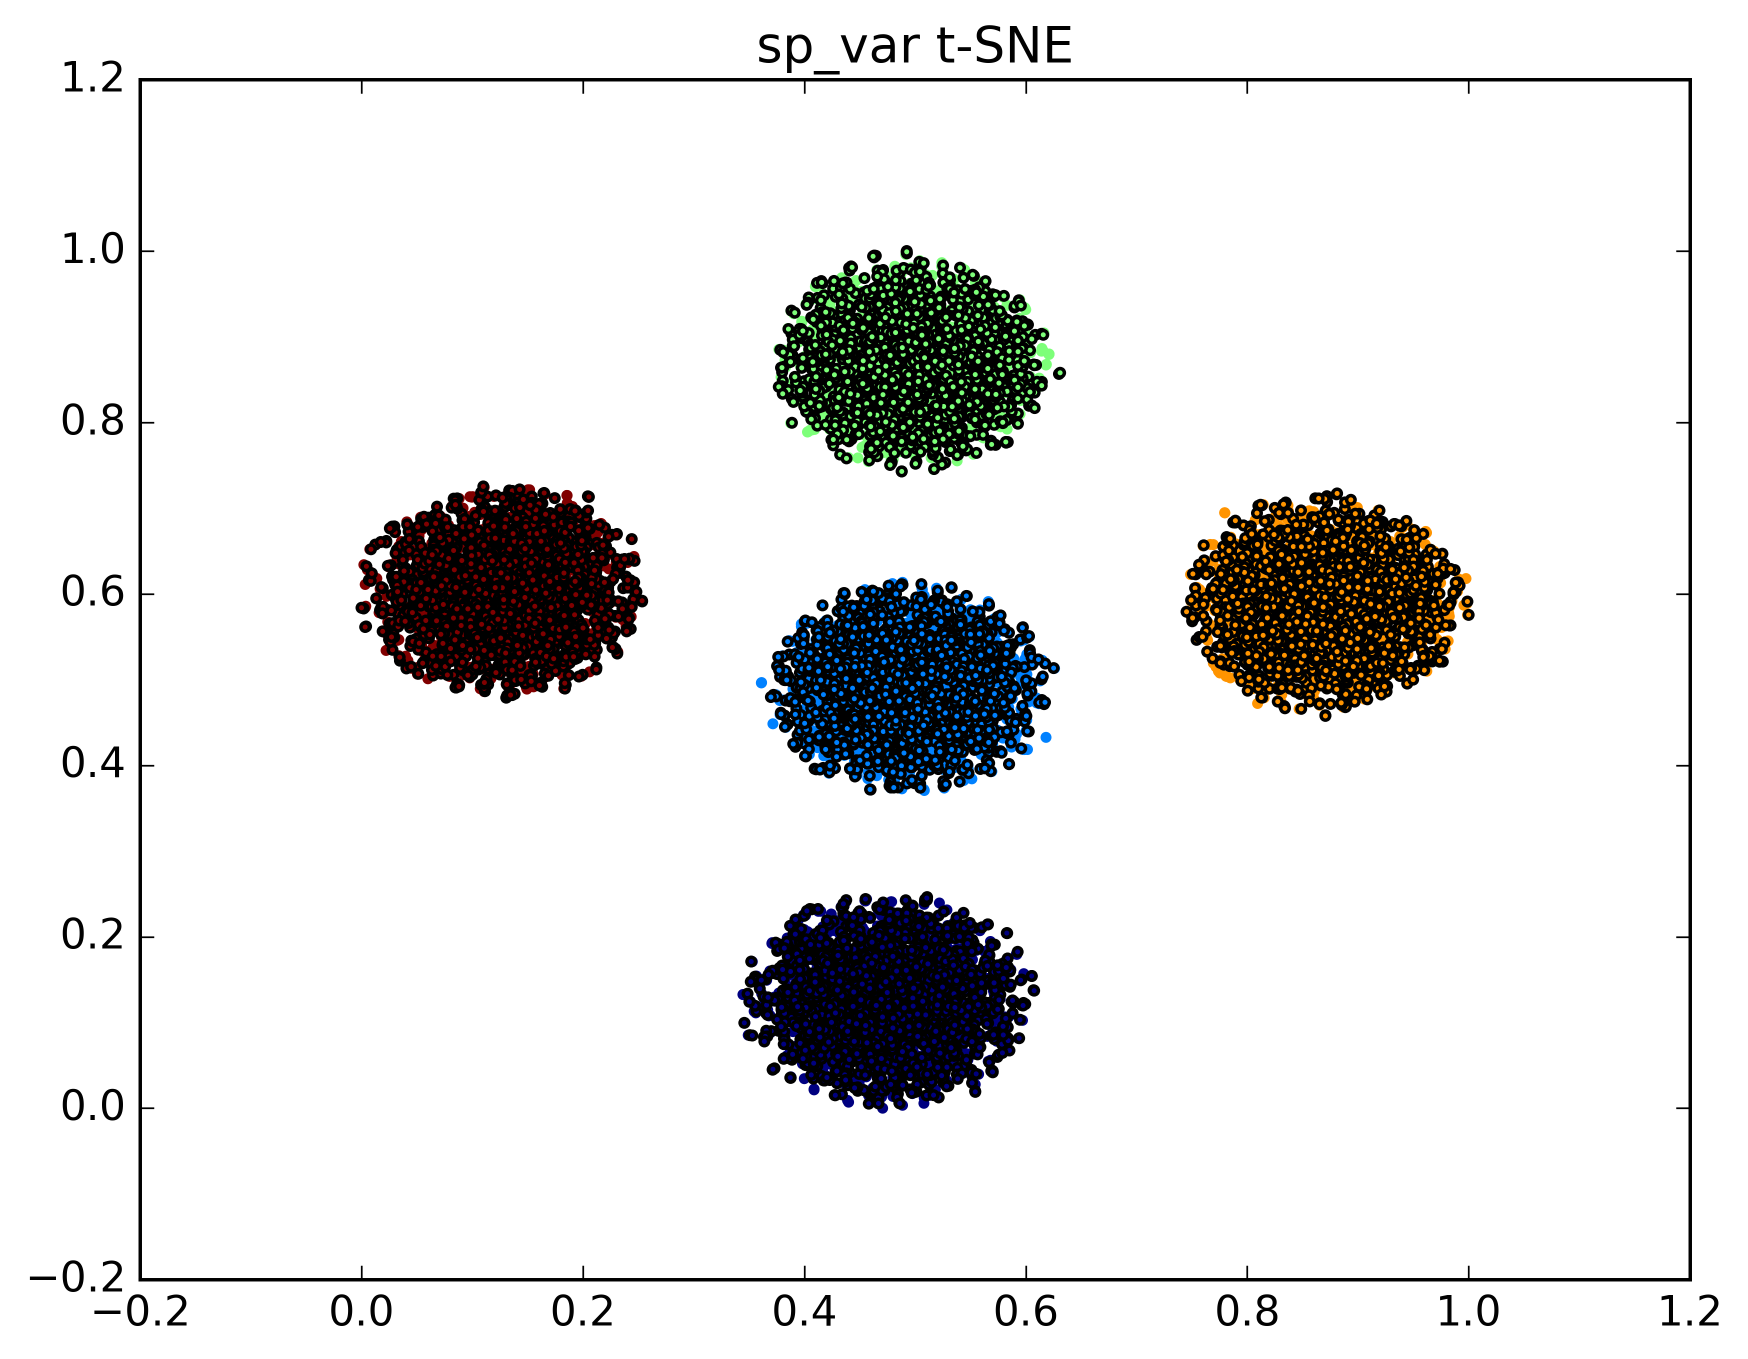
\includegraphics[width=1.0\textwidth]{sp_varu.png}
		\caption{Normalizing sp\_var as one unit}
		\label{fig:sp_var_nT}
	\end{minipage}\hfill
	\begin{minipage}{0.5\textwidth}
		\centering
		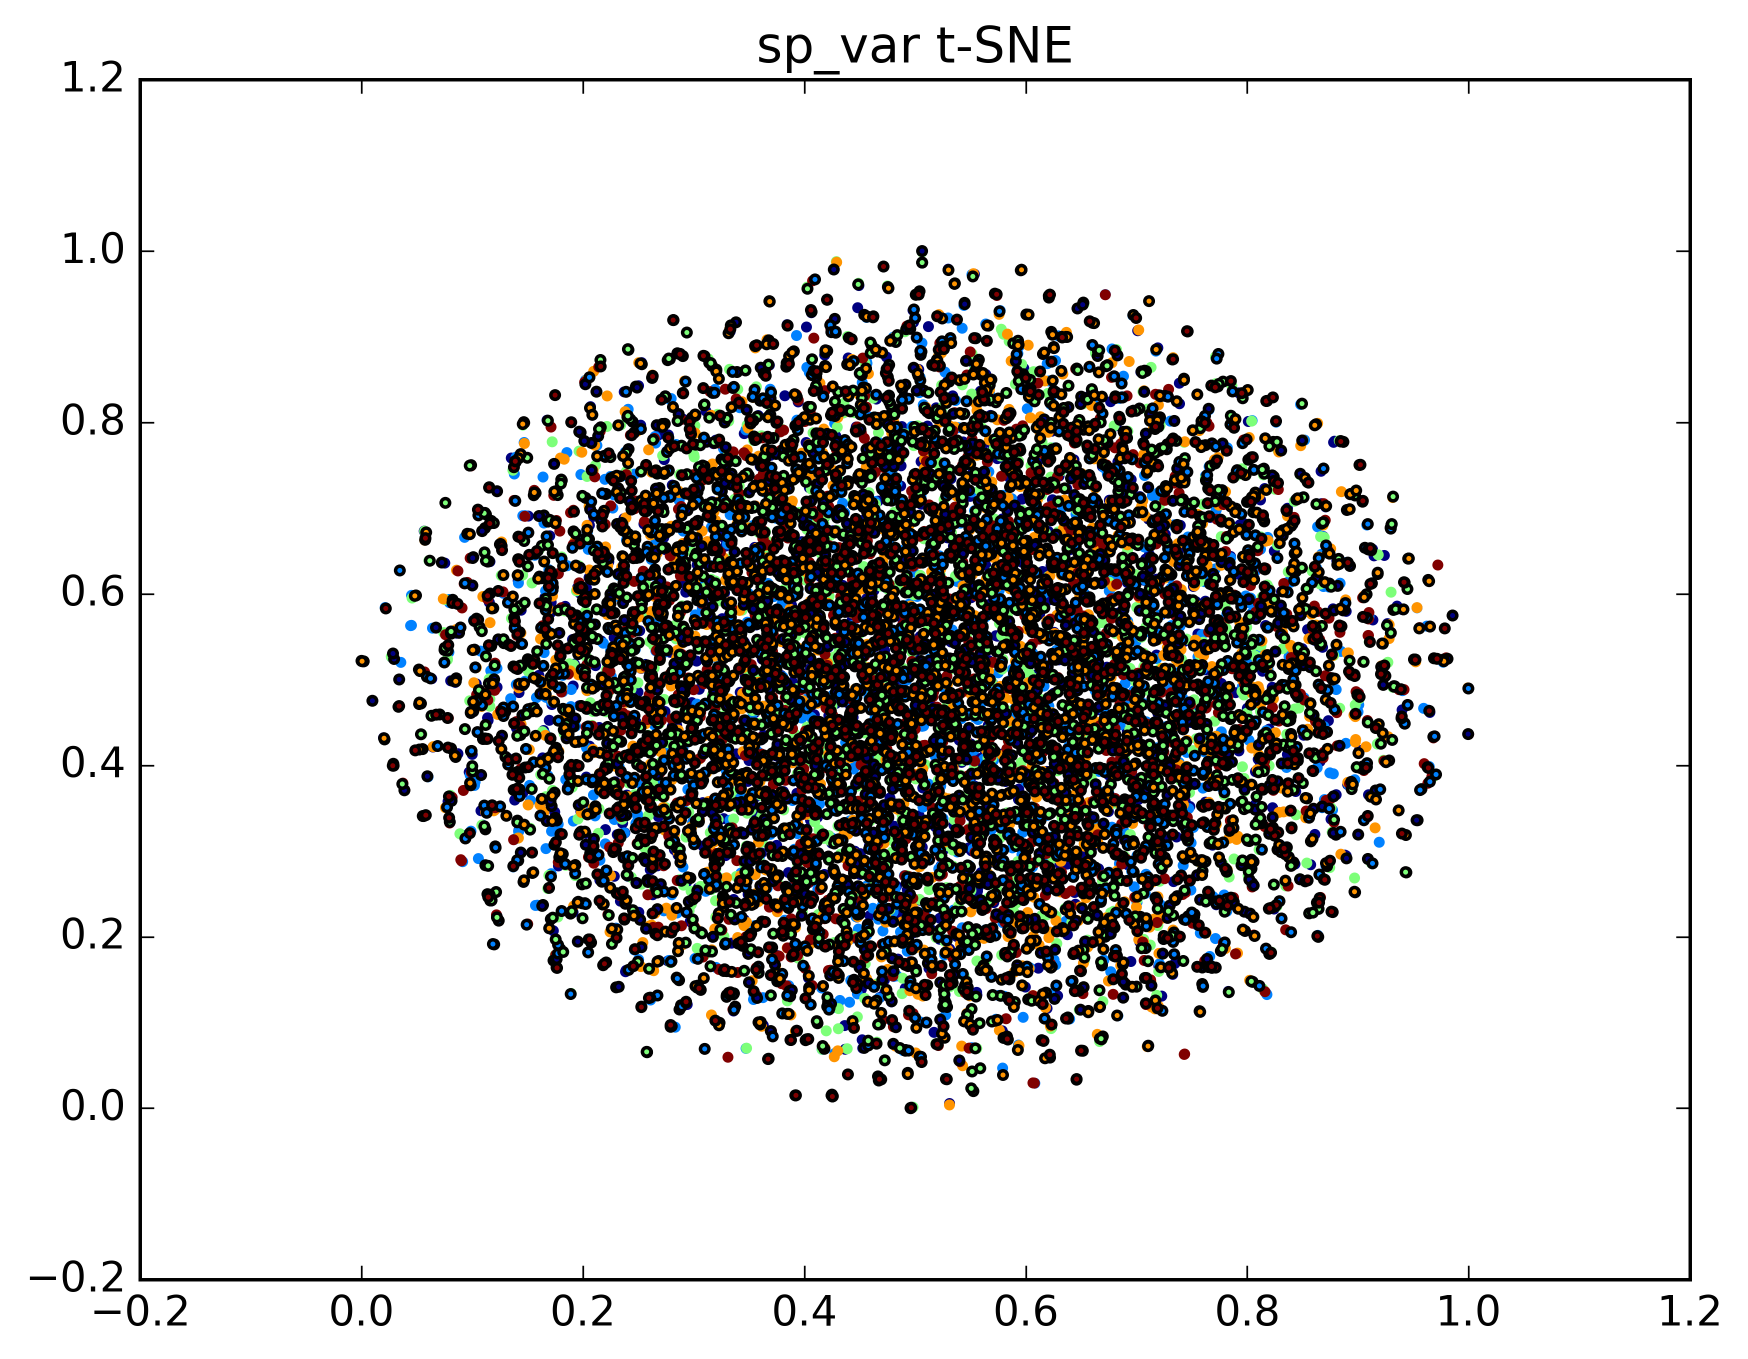
\includegraphics[width=1.0\textwidth]{sp_vart.png}
		\caption{Normalizing sp\_var trial-wise}
		\label{fig:sp_var_nF}
	\end{minipage}
\end{figure}
\begin{figure}[h]
	\centering
	\hspace*{-1.7cm}
	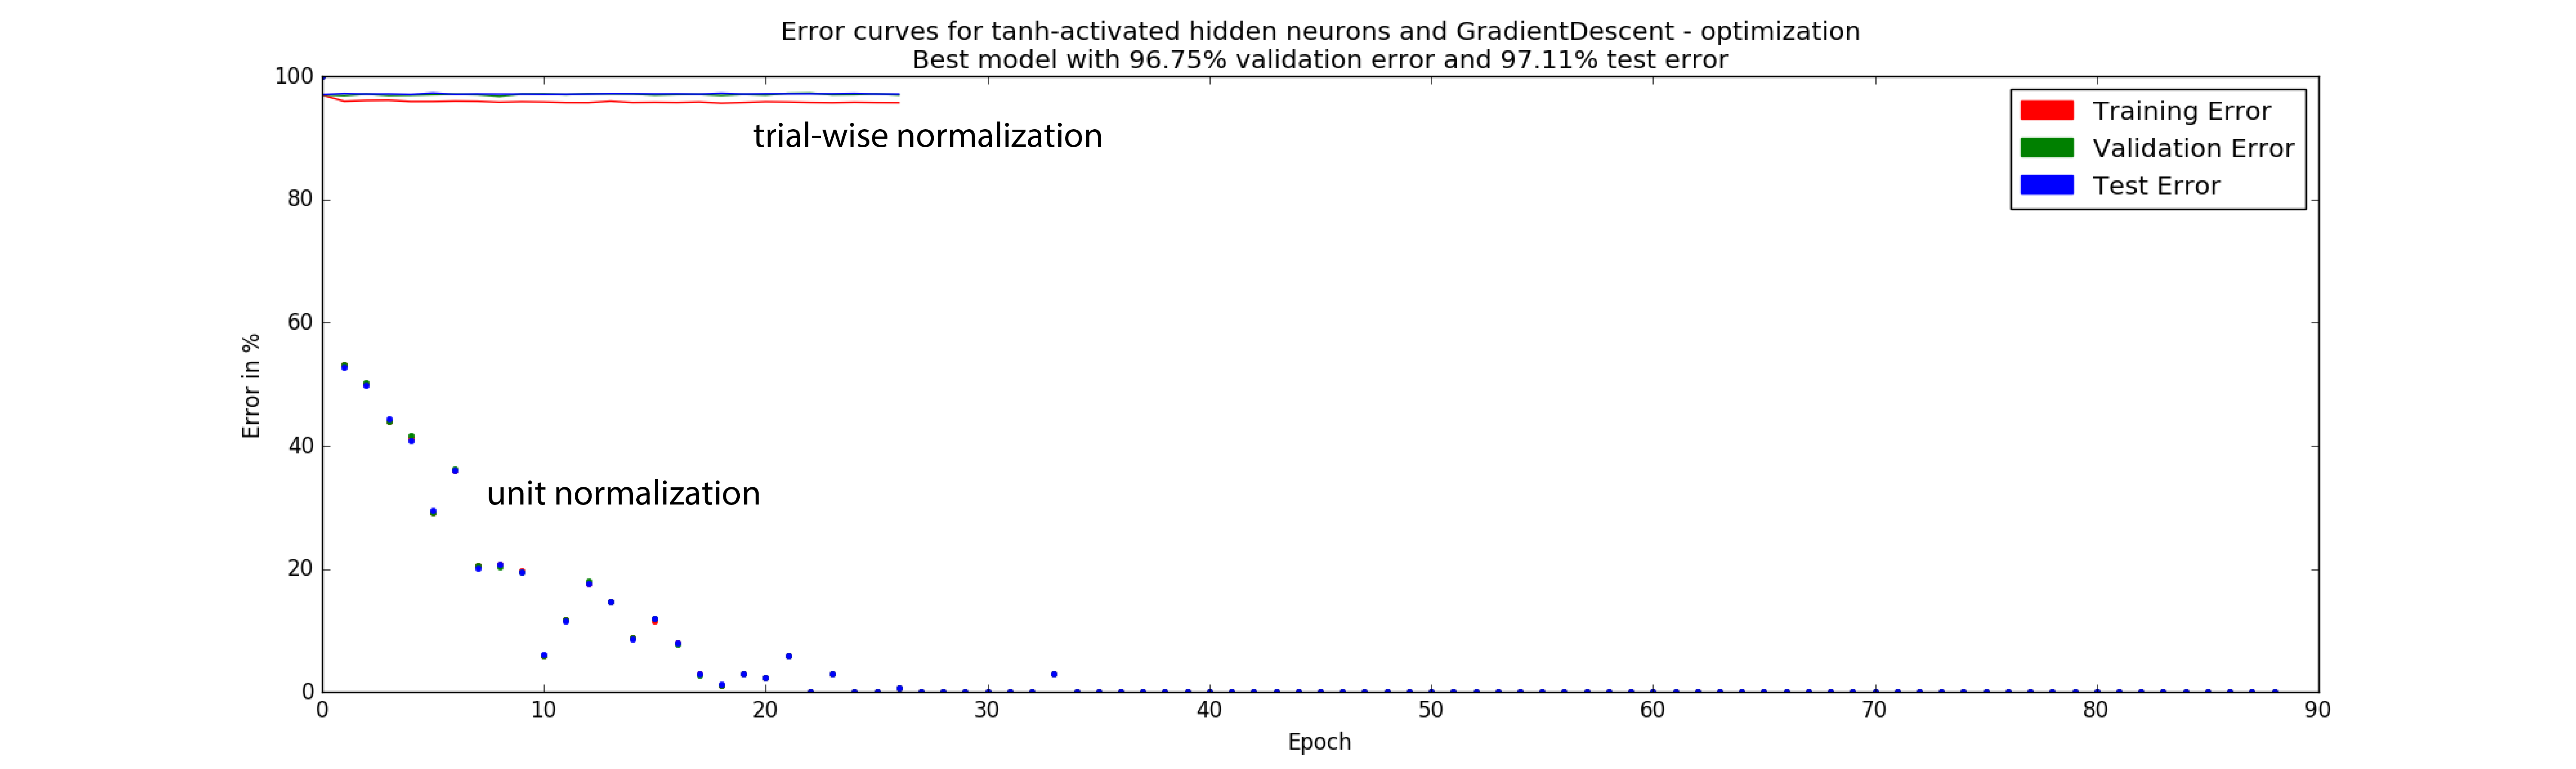
\includegraphics[width=1.25\textwidth]{sp_var_double.png}
	\caption{Neural net runs on sp\_var}
	\label{fig:sp_var_double}
\end{figure}

\section{Applying trial-wise normalization on real data}
Now, the t-SNE and neural net runs were once more to be applied to a selection of the datasets, expecting similar behaviour as that of \verb|sp_var|. However, things turned again out to be rather surprising.

\subsection{Participant 9, Series 5}
\begin{figure}
	\centering
	\begin{minipage}{0.5\textwidth}
		\centering
		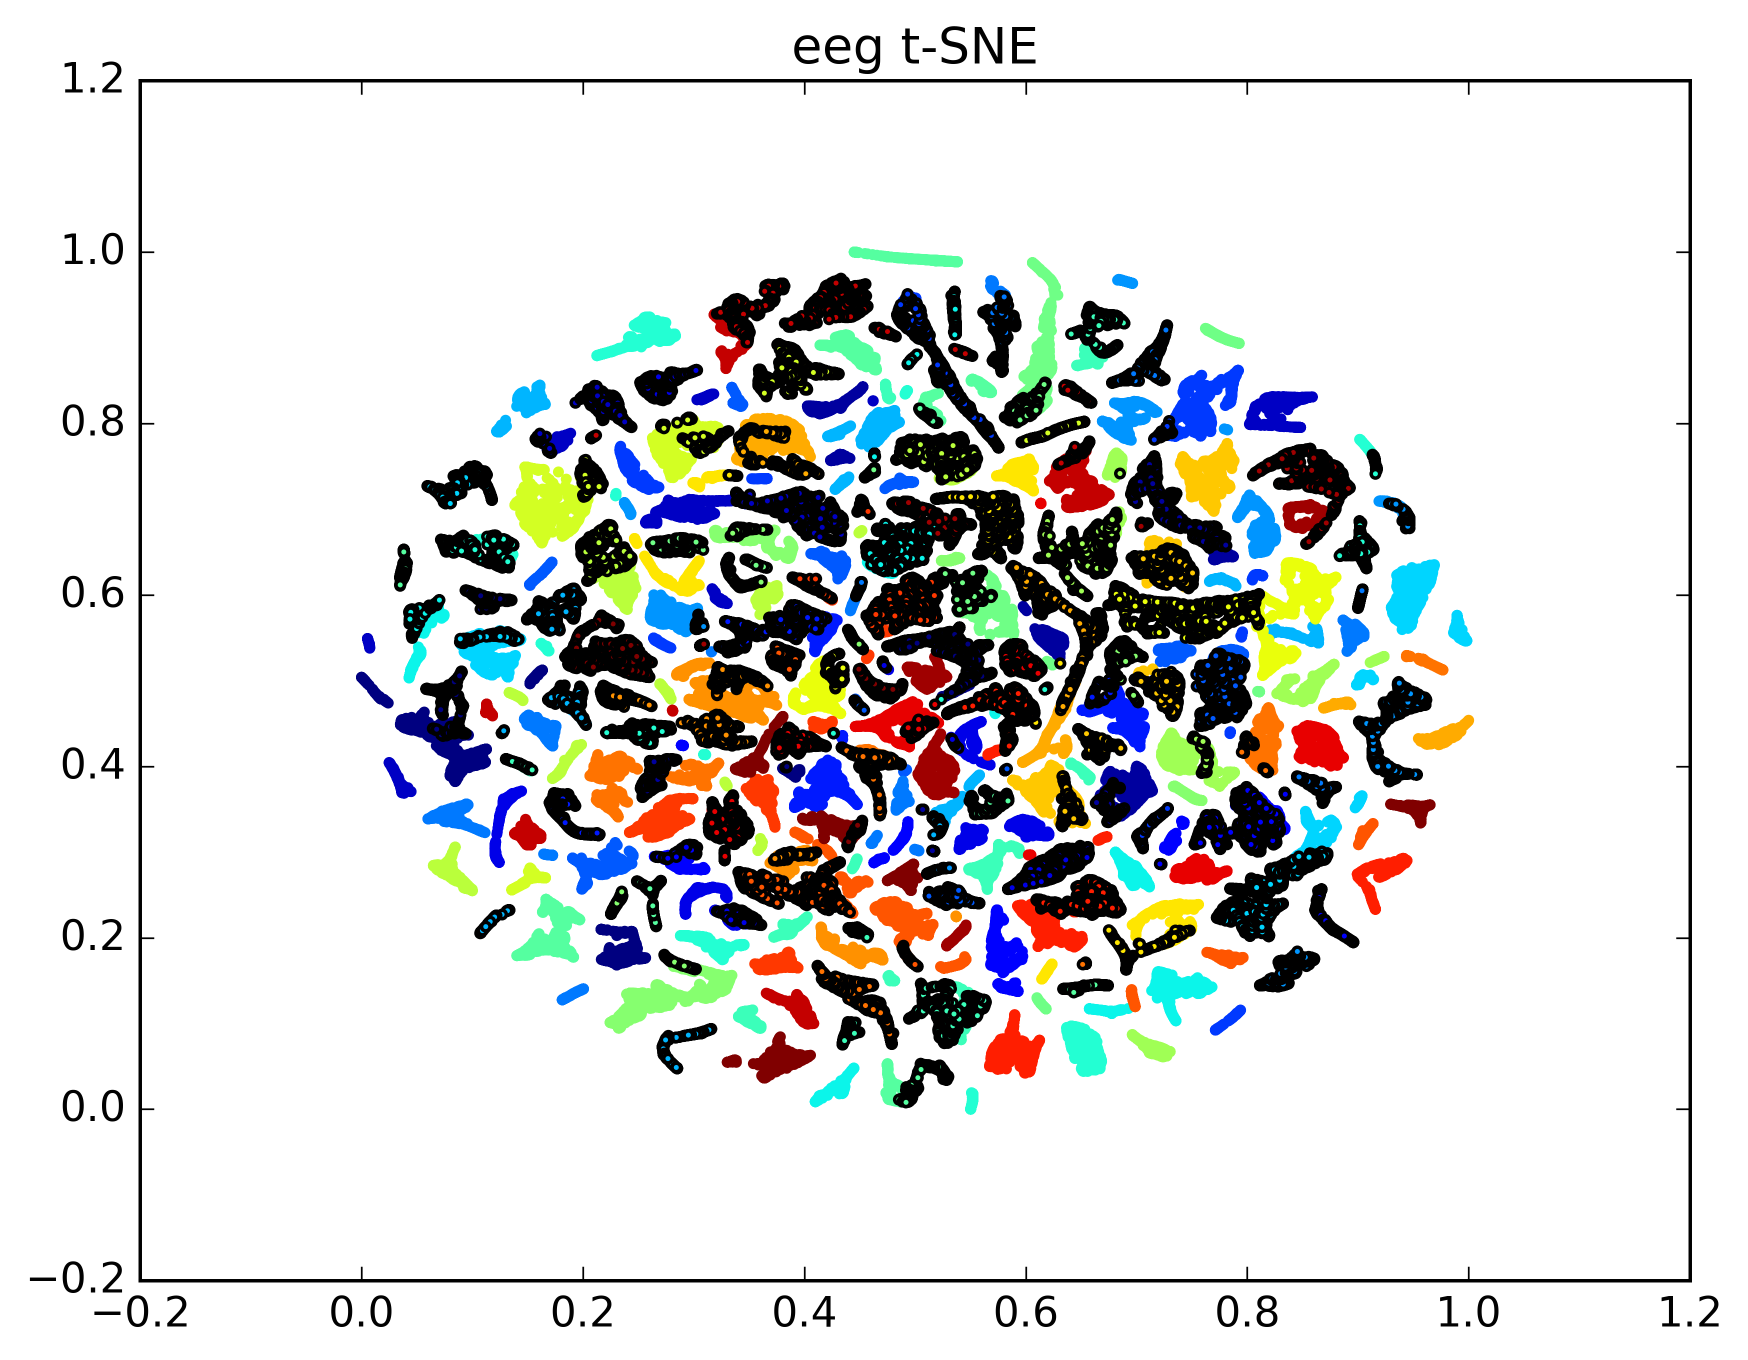
\includegraphics[width=1.0\textwidth]{P9S5u.png}
		\caption{Normalizing participant 9, series 5 as one unit}
		\label{fig:P9S5u}
	\end{minipage}\hfill
	\begin{minipage}{0.5\textwidth}
		\centering
		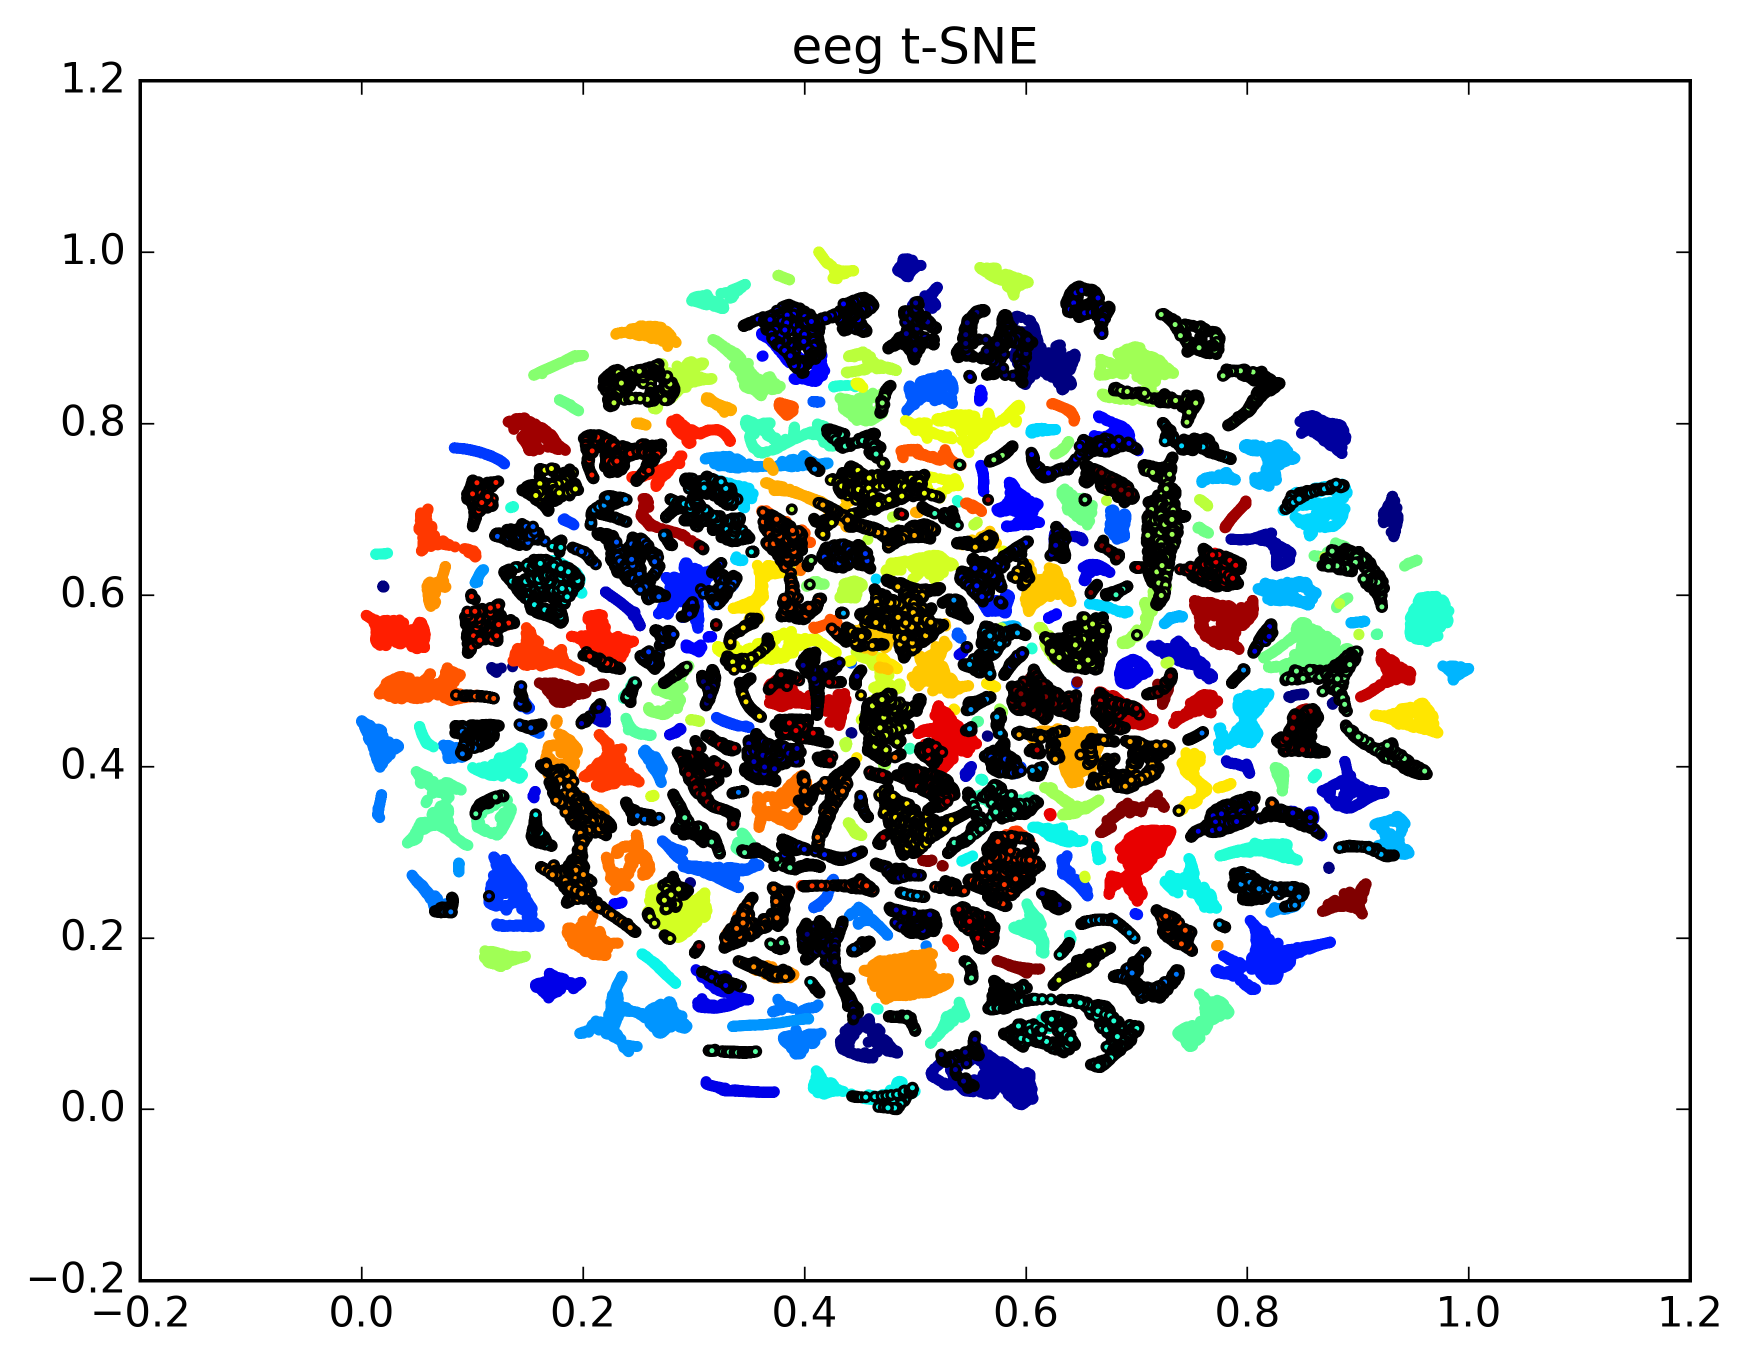
\includegraphics[width=1.0\textwidth]{P9S5t.png}
		\caption{Normalizing participant 9, series 5 trial-wise}
		\label{fig:P9S5t}
	\end{minipage}
\end{figure}
\begin{figure}[h]
	\centering
	\hspace*{-1.7cm}
	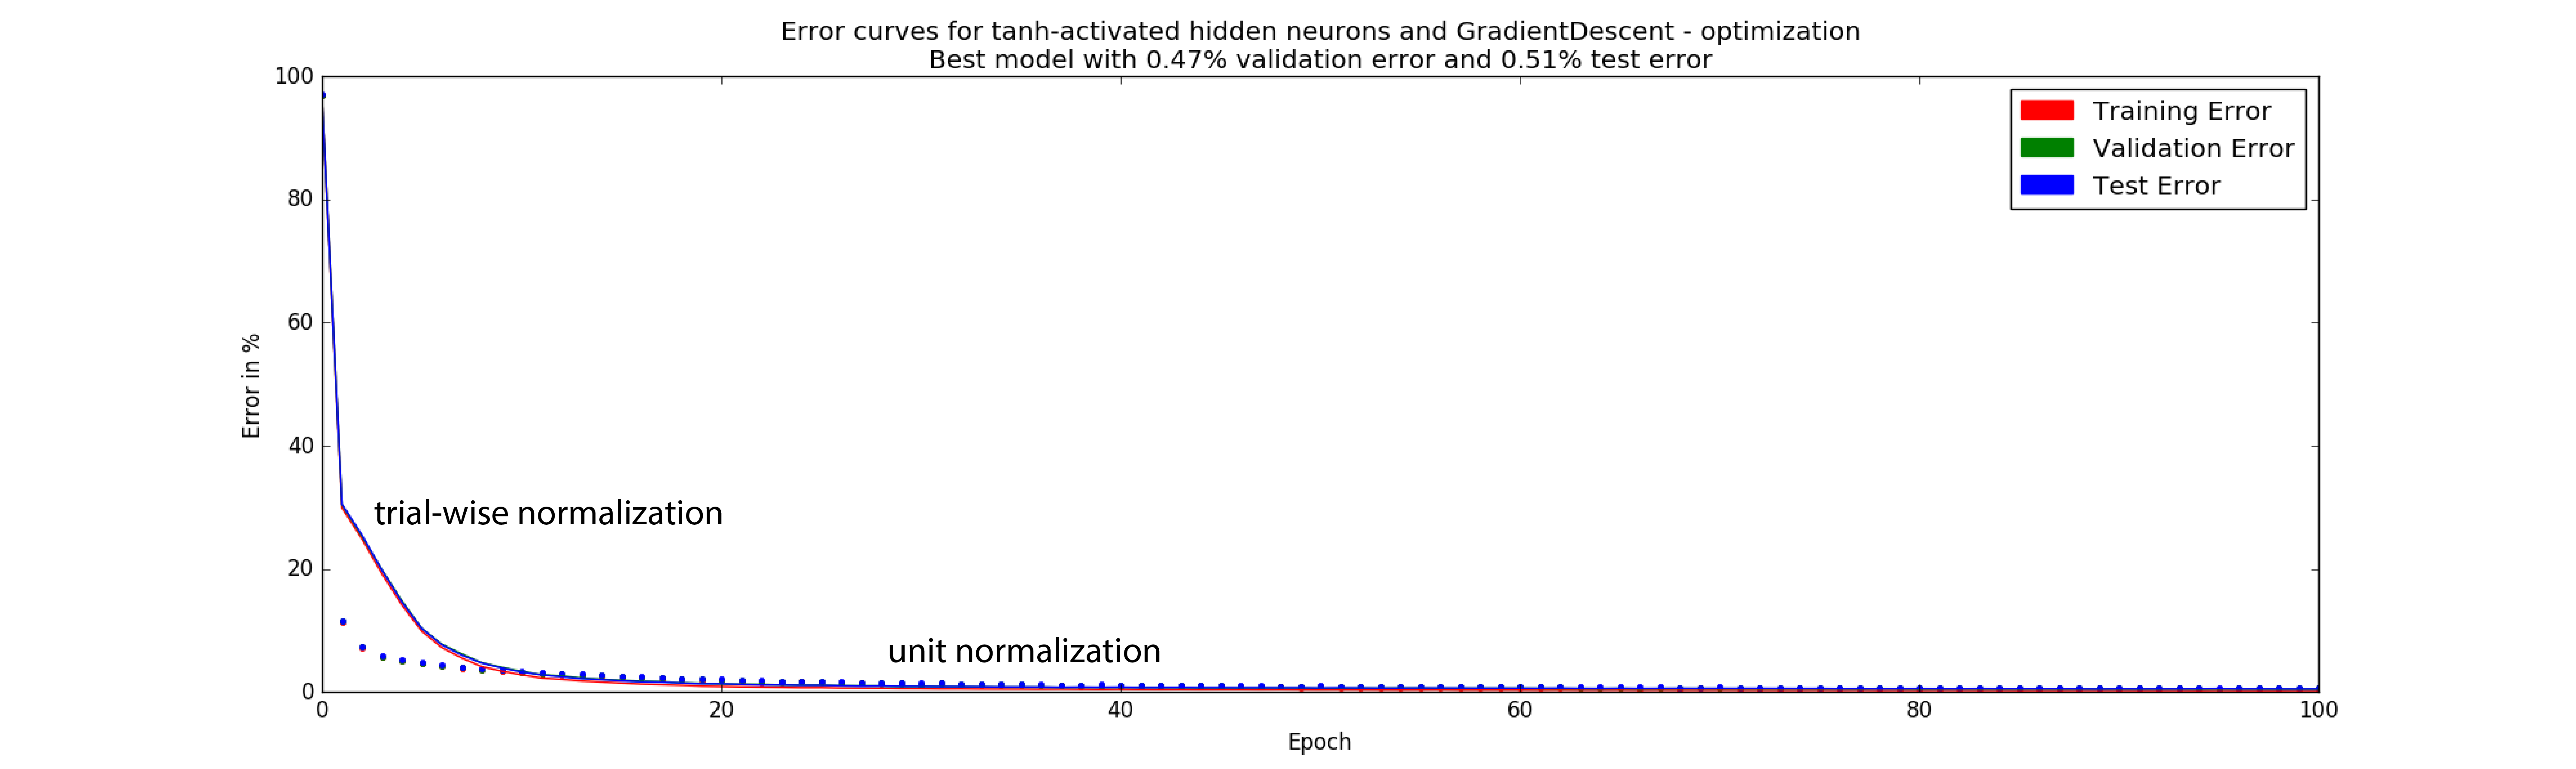
\includegraphics[width=1.25\textwidth]{P9S5_double.png}
	\caption{Neural net runs on participant 9, series 5}
	\label{fig:P9S5_double}
\end{figure}
First, the data belonging to participant 9, series 5 was tested as this achieved the most extreme test error of $0.03\%$ in previous neural net runs. The results of the t-SNE runs are shown in figure \ref{fig:P9S5u} for unit-normalization and in figure \ref{fig:P9S5t} for trial-wise normalization, respectively. Surprisingly, both results barely differ. On the neural net run, the unit-normalized version this time achieved \emph{only} an error of $0.61\%$. With trial-wise normalization this result was beaten with a slightly better error of $0.51\%$. Figure \ref{fig:P9S5_double} shows the achieved error rates.


\subsection{Participant 1, Series 1}
\begin{figure}
	\centering
	\begin{minipage}{0.5\textwidth}
		\centering
		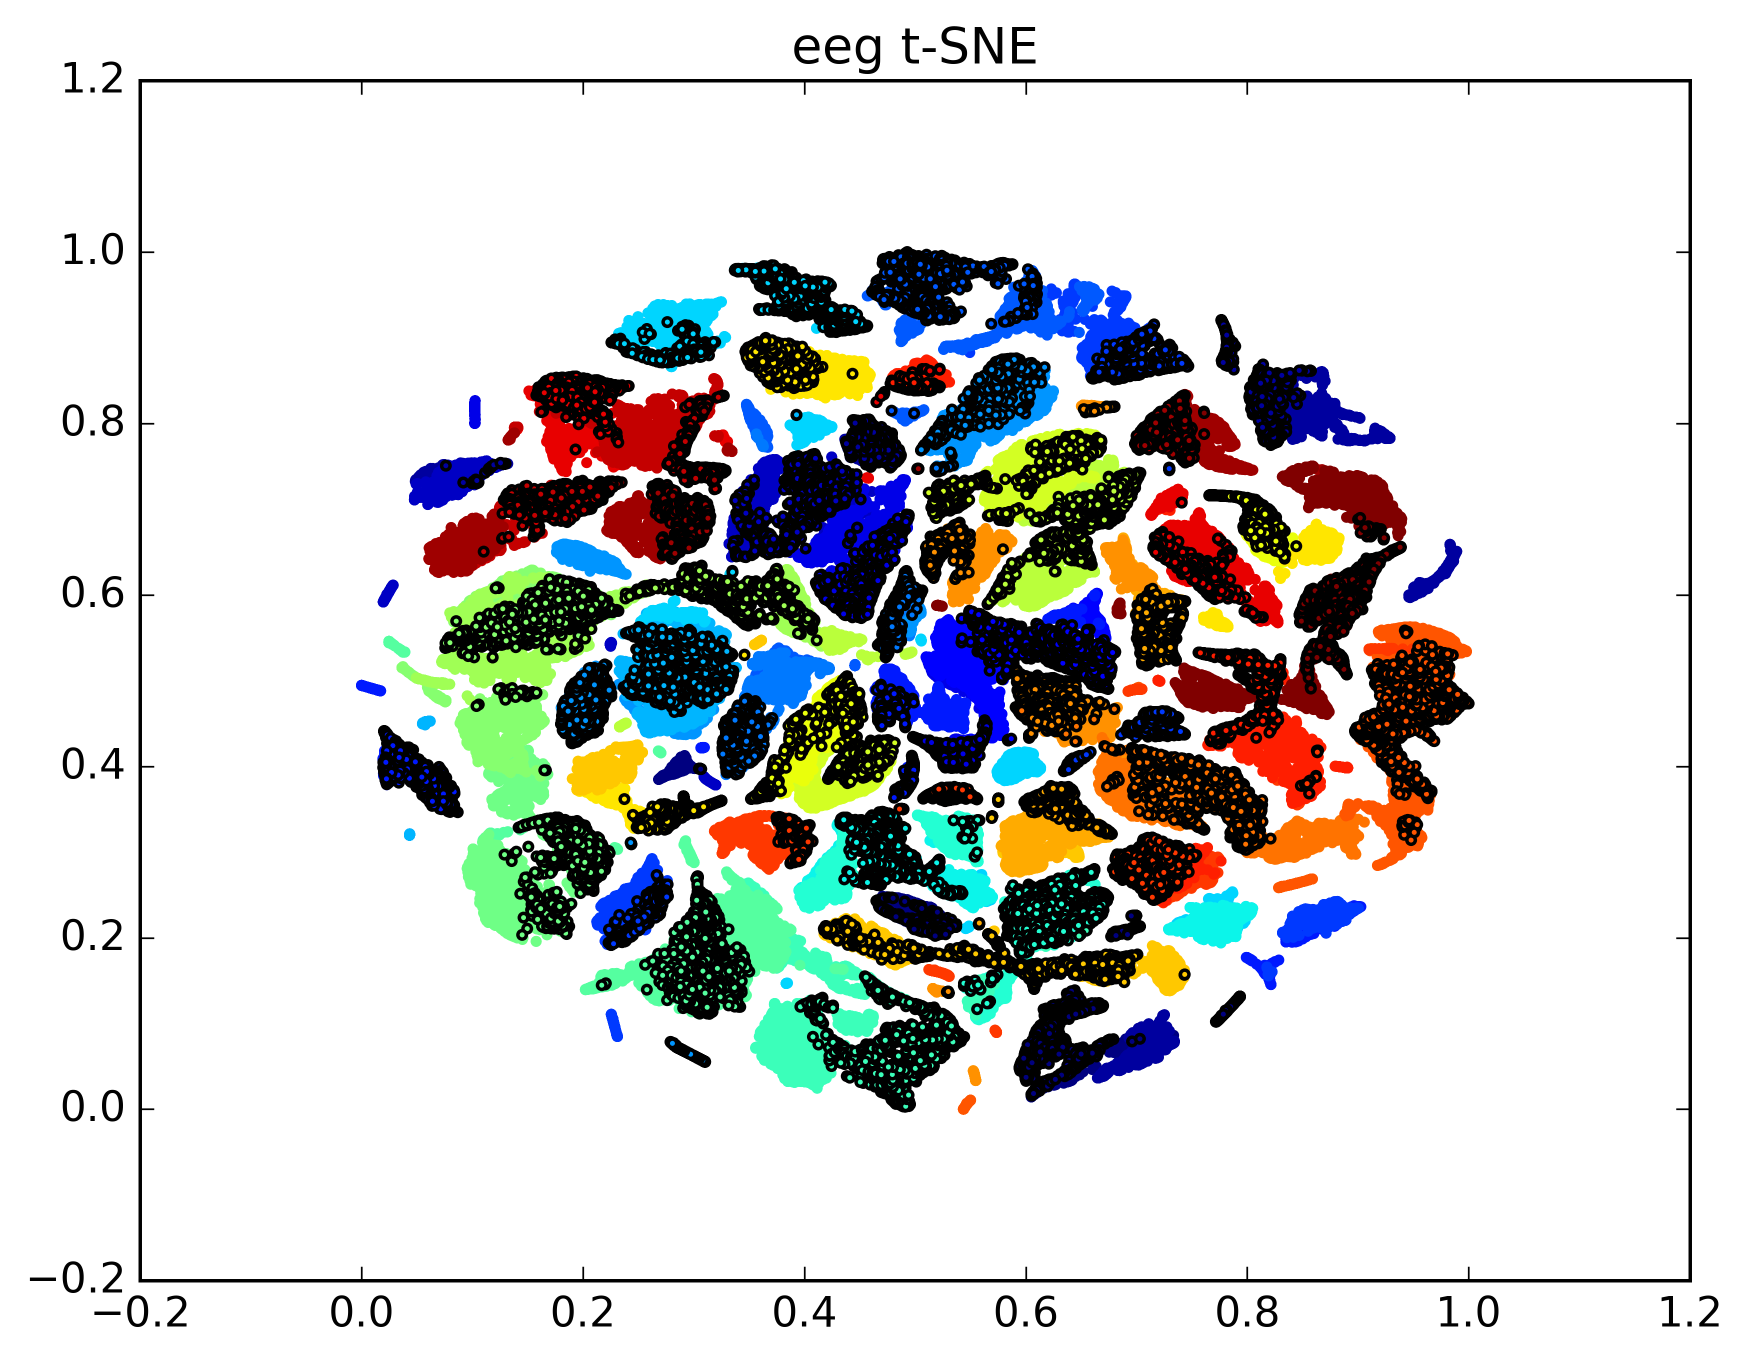
\includegraphics[width=1.0\textwidth]{P1S1u.png}
		\caption{Normalizing participant 1, series 1 as one unit}
		\label{fig:P1S1u}
	\end{minipage}\hfill
	\begin{minipage}{0.5\textwidth}
		\centering
		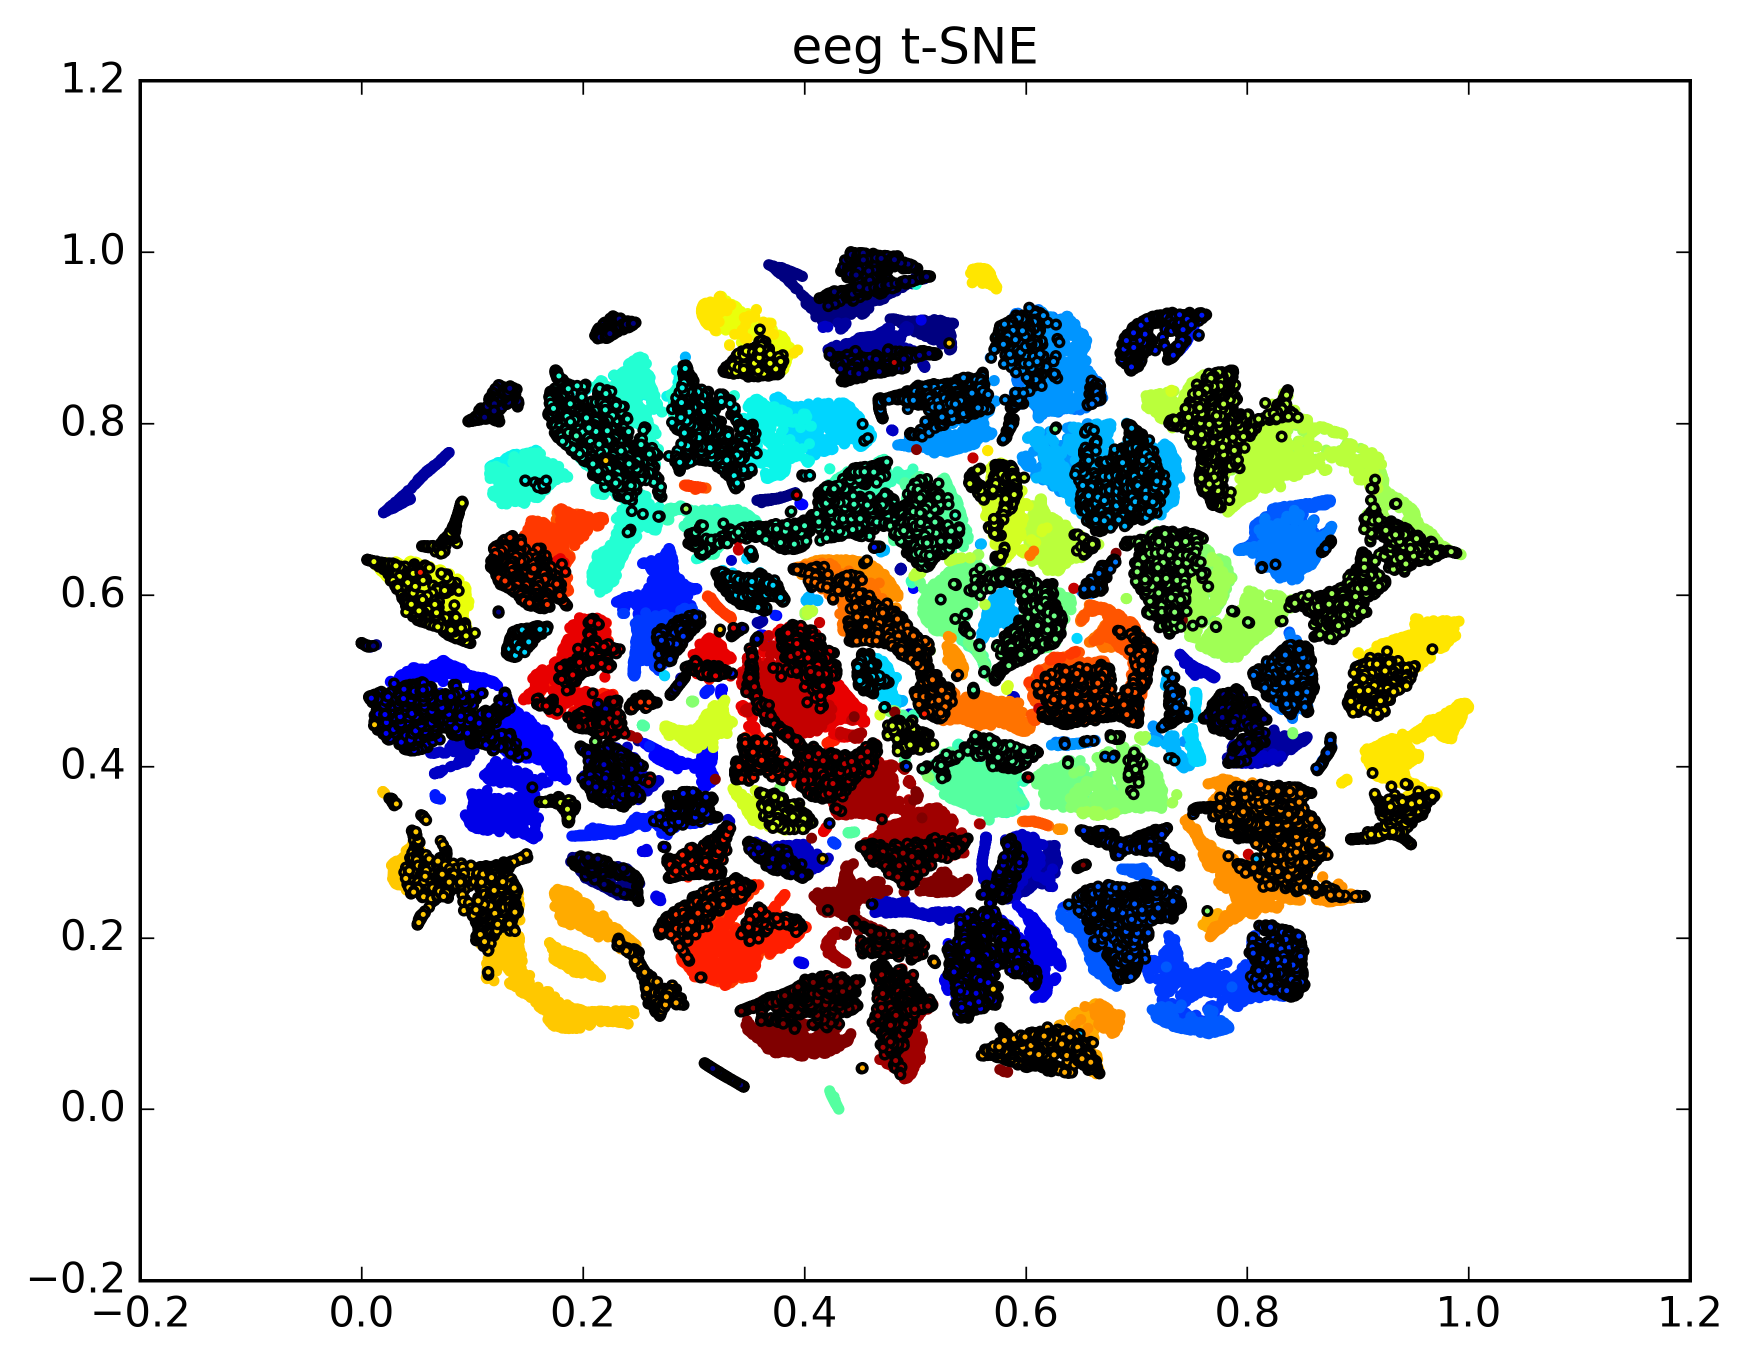
\includegraphics[width=1.0\textwidth]{P1S1t.png}
		\caption{Normalizing participant 1, series 1 trial-wise}
		\label{fig:P1S1t}
	\end{minipage}
\end{figure}
\begin{figure}[h]
	\centering
	\hspace*{-1.7cm}
	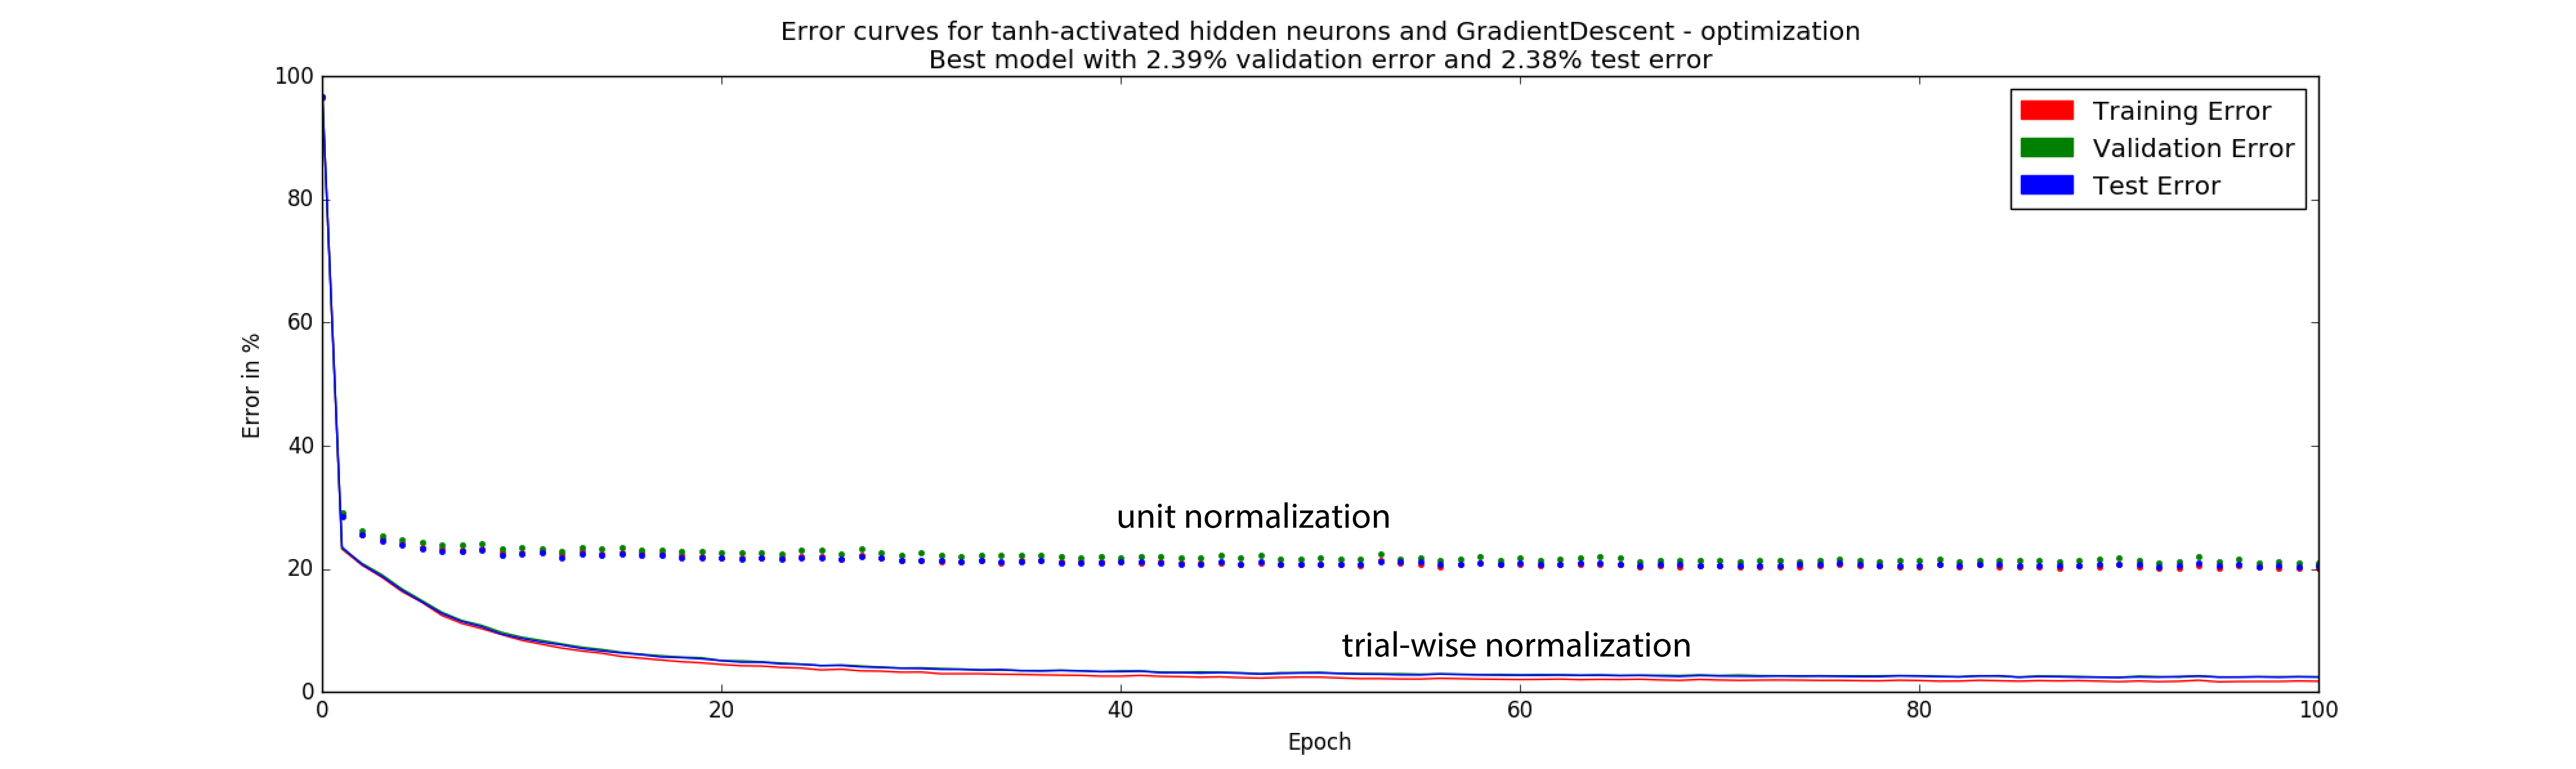
\includegraphics[width=1.25\textwidth]{P1S1_double.png}
	\caption{Neural net runs on participant 1, series 1}
	\label{fig:P1S1_double}
\end{figure}
Then, the dataset of participant 1, series 1 was tested. The results of the t-SNE runs are shown in figure \ref{fig:P1S1u} for unit-normalization and in figure \ref{fig:P1S1t} for trial-wise normalization, respectively. Again, both results barely differ. The neural net test revealed much more interesting results, however. Before, using unit-normalization, a test error of just below $20\%$ was achieved. When using trial-wise normalization the error rate actually improved significantly, reaching mere $2.38\%$. The corresponding error rates are plotted in figure \ref{fig:P1S1_double}.



\subsection{Participant 7, Series 8}
\begin{figure}
	\centering
	\begin{minipage}{0.5\textwidth}
		\centering
		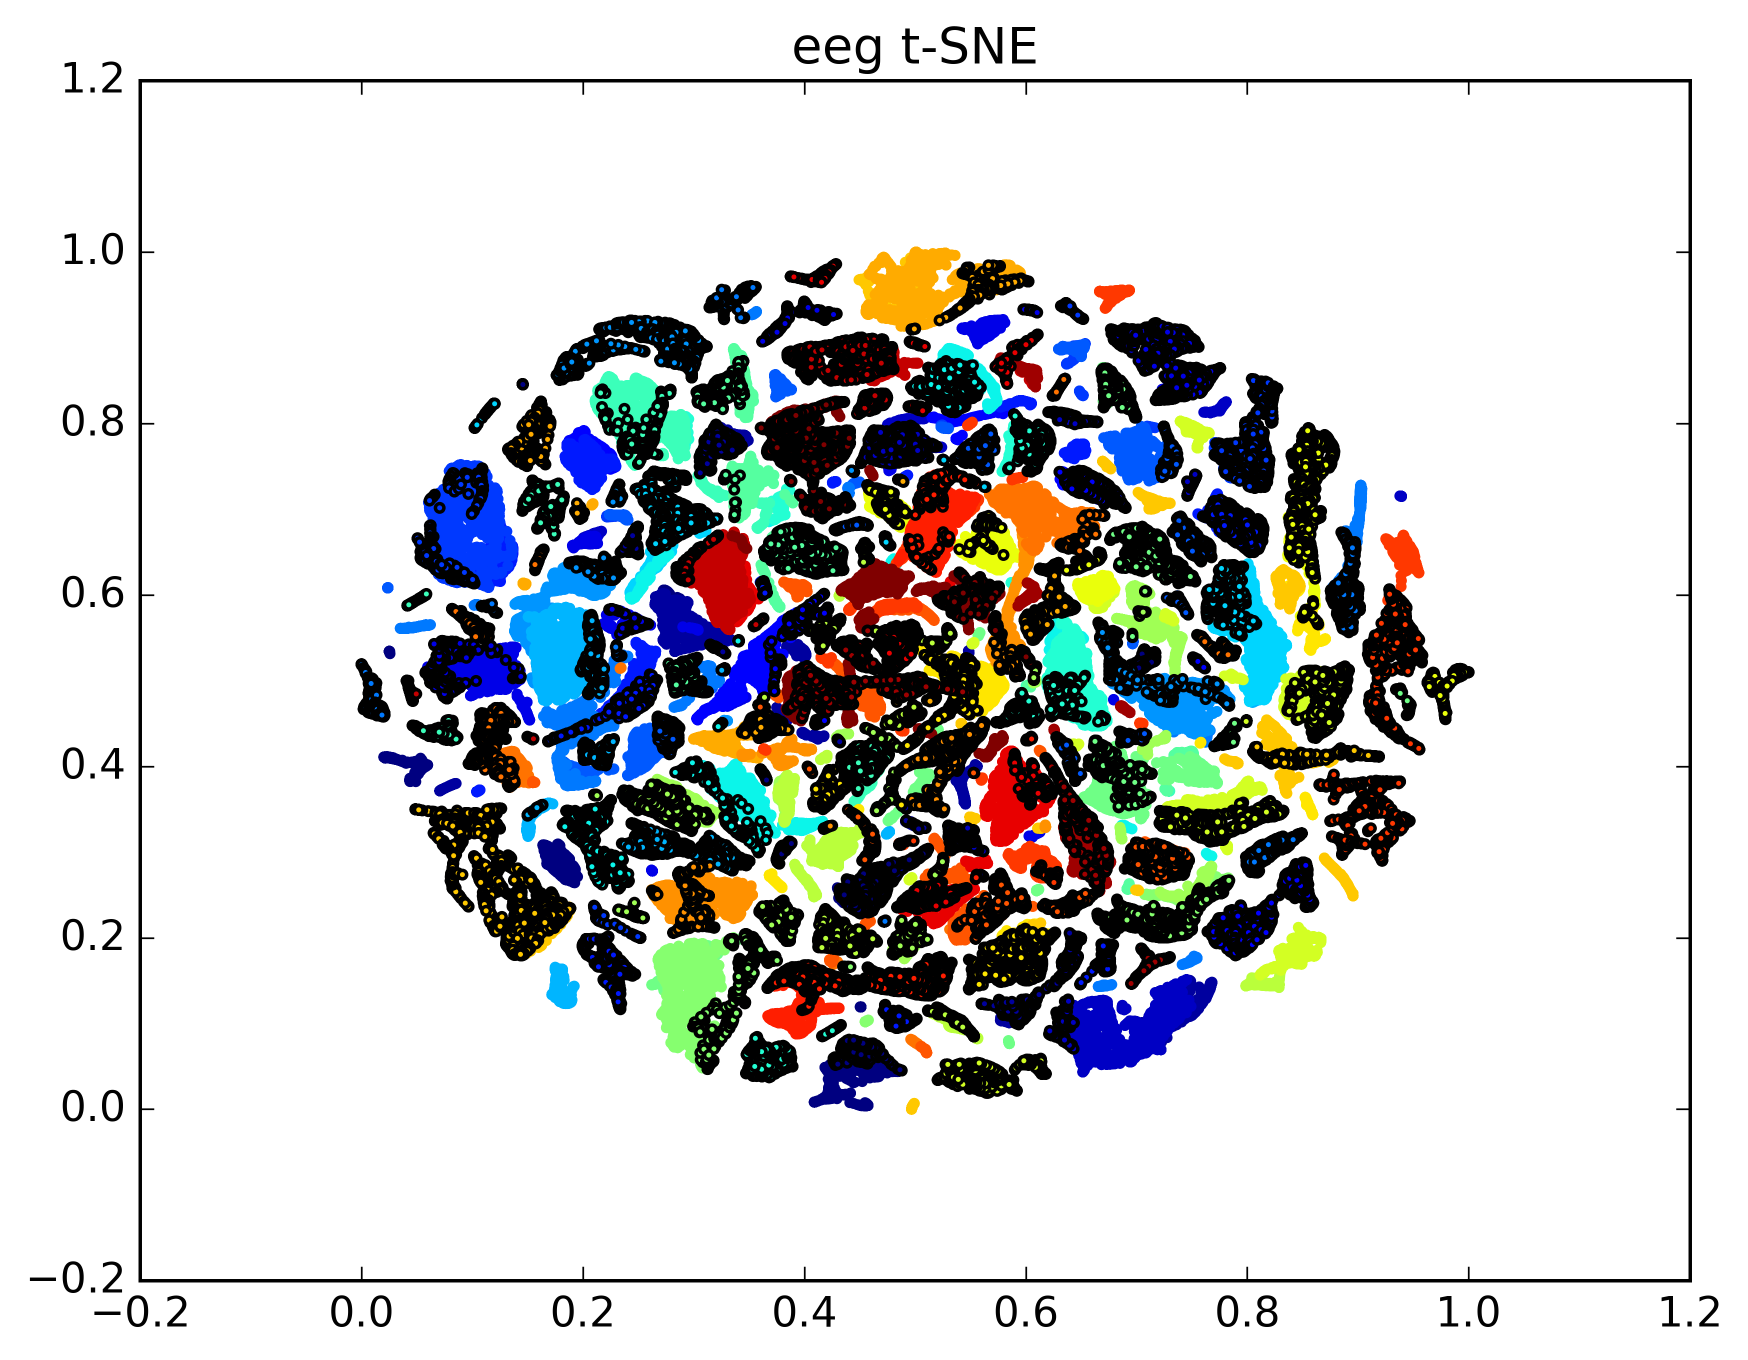
\includegraphics[width=1.0\textwidth]{P7S8u.png}
		\caption{Normalizing participant 7, series 8 as one unit}
		\label{fig:P7S8u}
	\end{minipage}\hfill
	\begin{minipage}{0.5\textwidth}
		\centering
		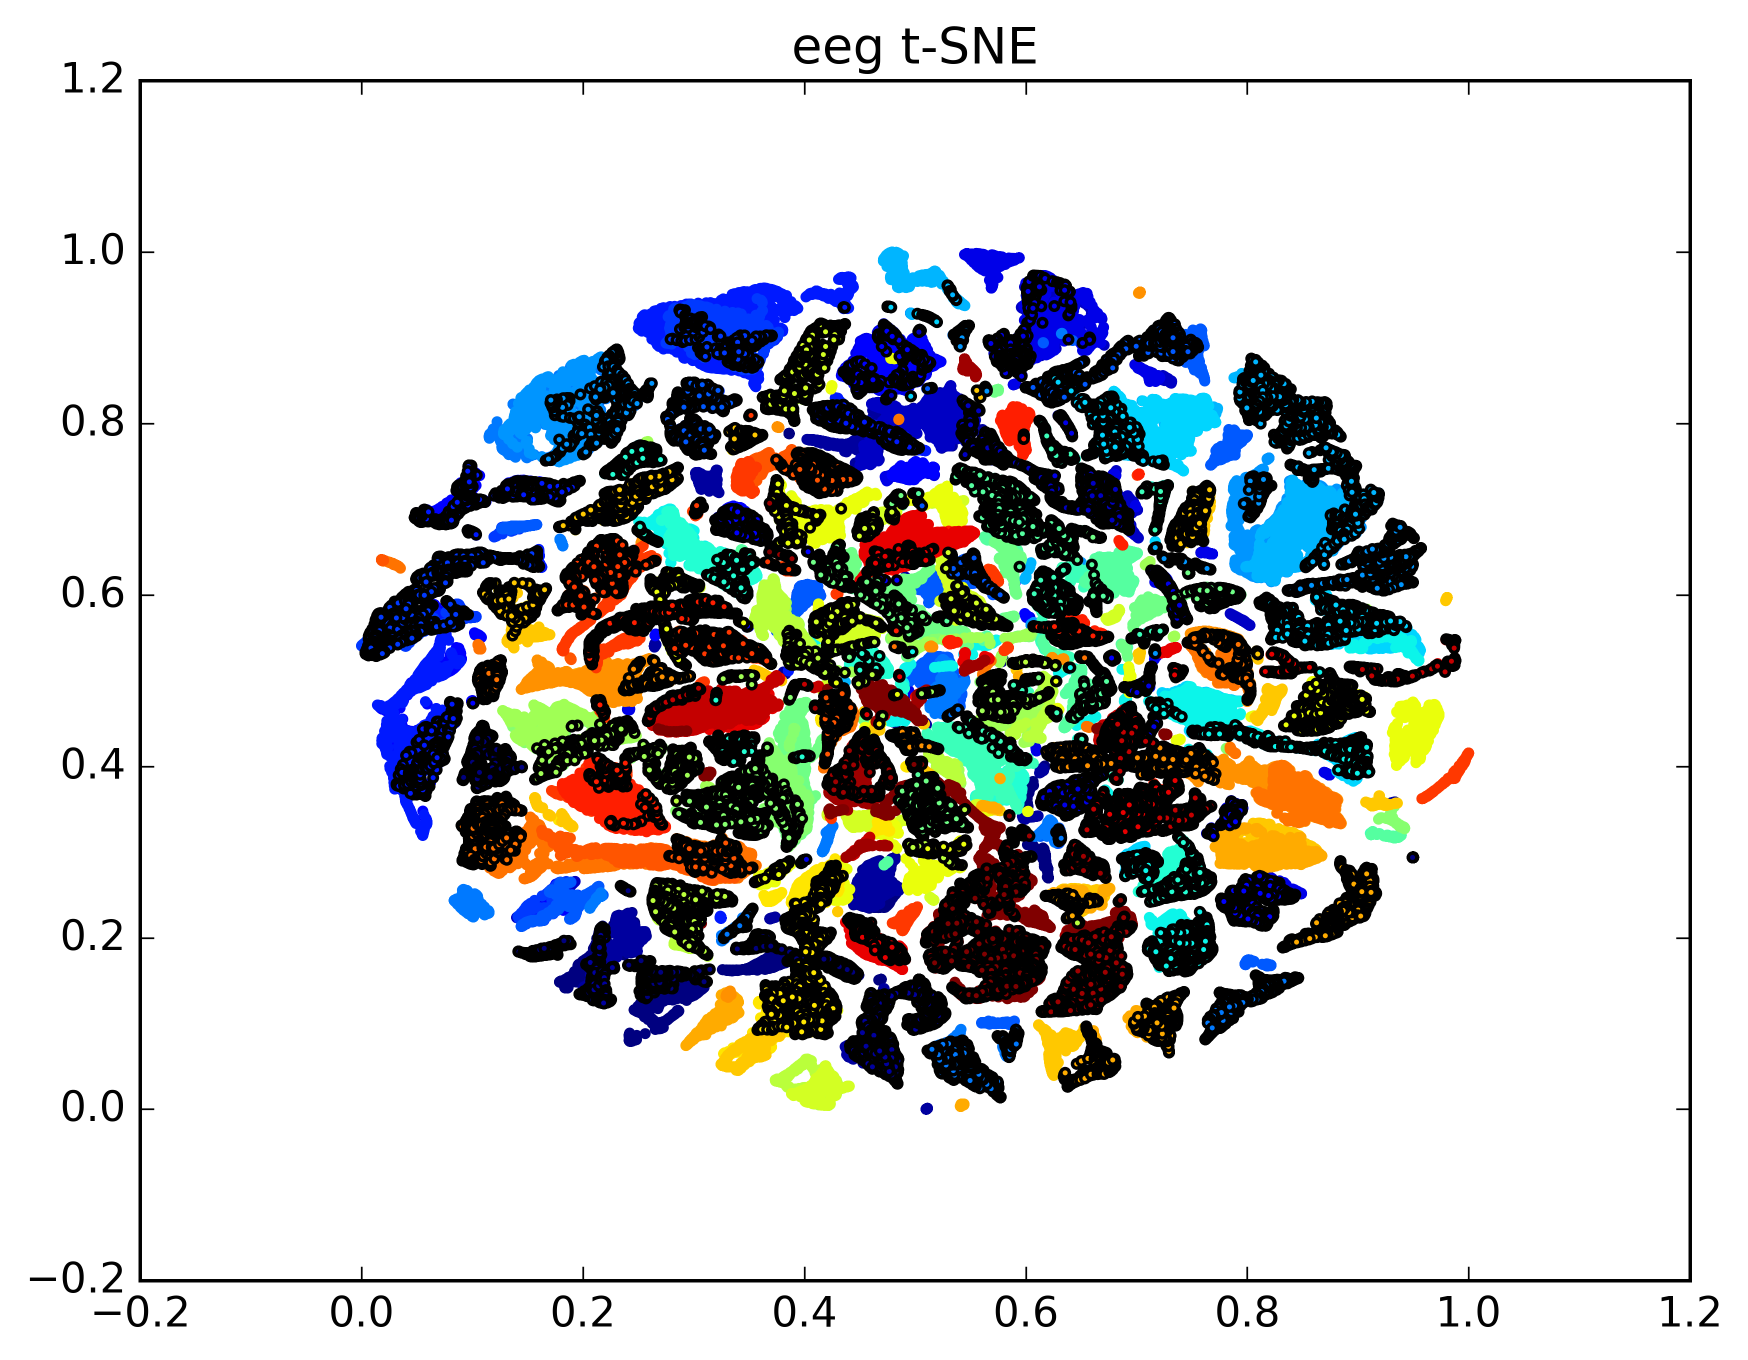
\includegraphics[width=1.0\textwidth]{P7S8t.png}
		\caption{Normalizing participant 7, series 8 trial-wise}
		\label{fig:P7S8t}
	\end{minipage}
\end{figure}
\begin{figure}[h]
	\centering
	\hspace*{-1.7cm}
	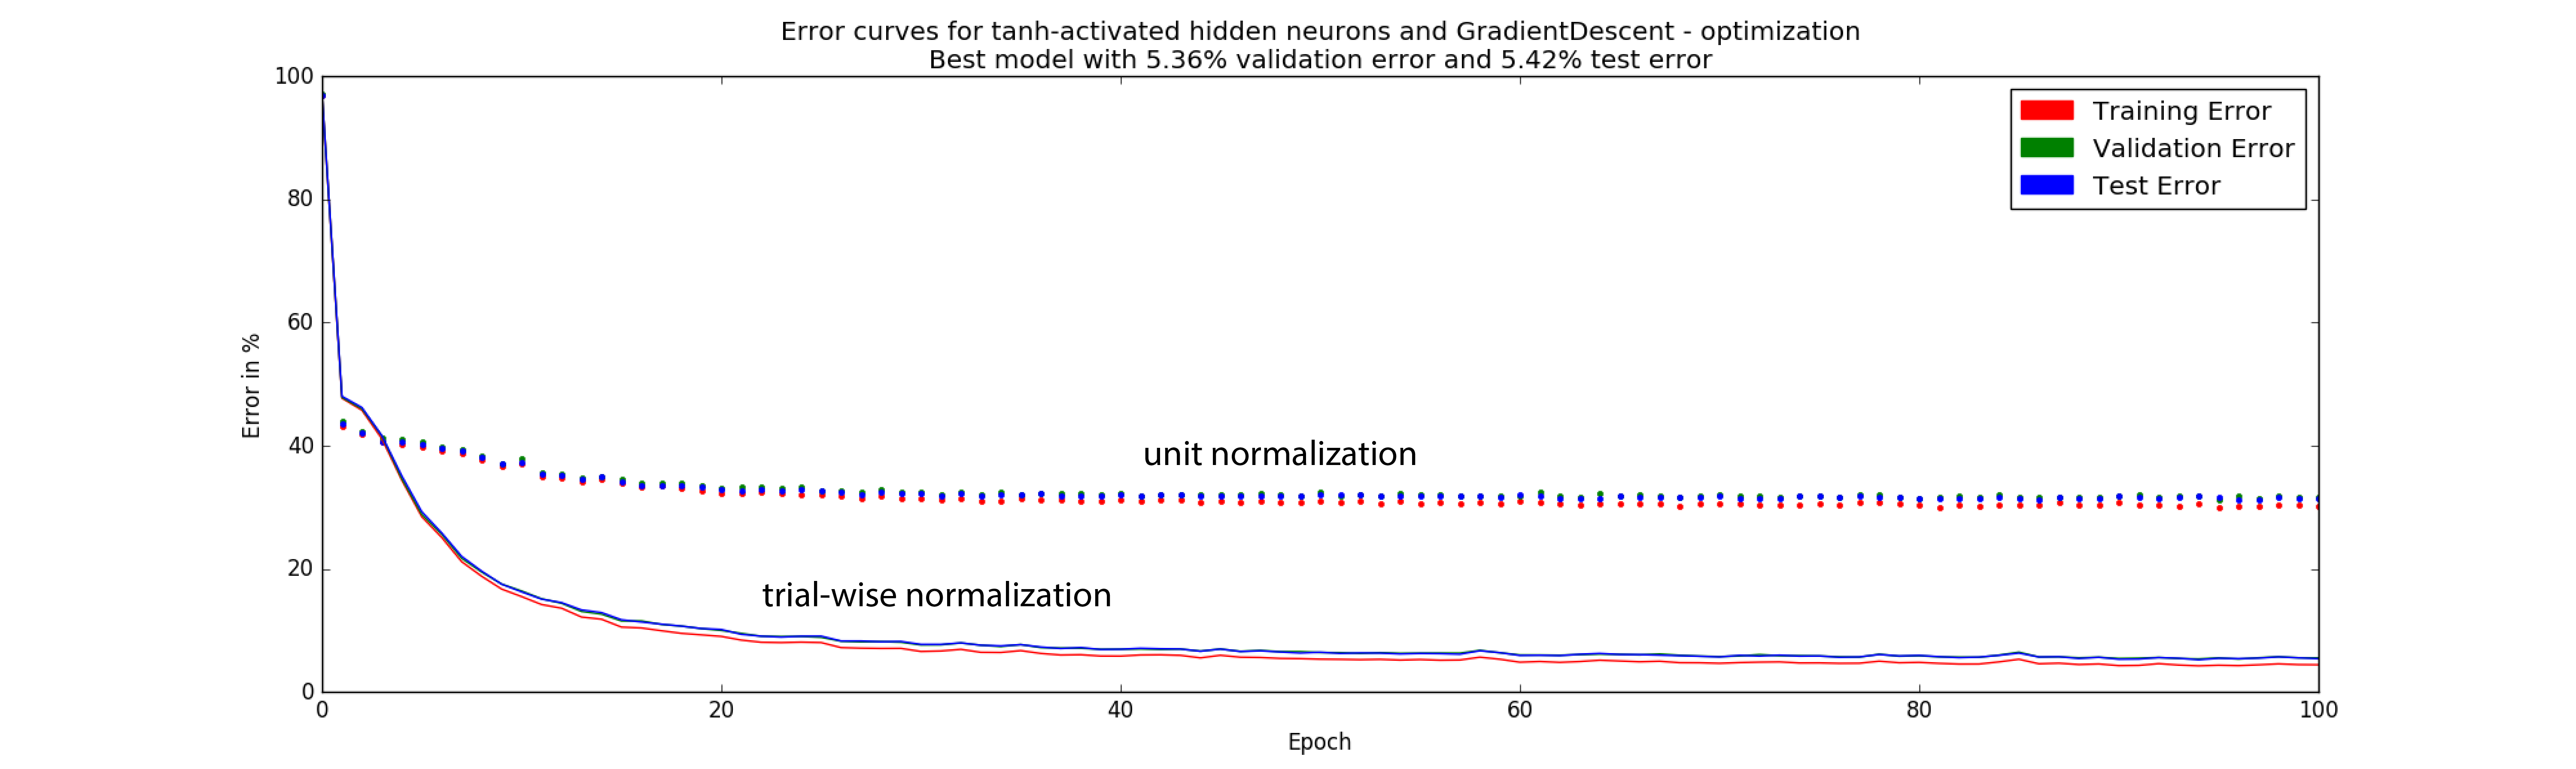
\includegraphics[width=1.25\textwidth]{P7S8_double.png}
	\caption{Neural net runs on participant 7, series 8}
	\label{fig:P7S8_double}
\end{figure}
At last, the dataset of participant 7, series 8 was tested. This dataset achieved the worst test error out of all the previously tested participants and series. As the trial-wise normalization made for such significant improvements on participant 1, series 1, it seemed interesting to examine if this would apply here, too. The results of the t-SNE runs are shown in figure \ref{fig:P7S8u} for unit-normalization and in figure \ref{fig:P7S8t} for trial-wise normalization, respectively. Once again, the two results look quite the same. The neural net error, though, improved upon the unit-normalized version indeed yet again. Using unit-normalization, a test error of just $31.57\%$ was achieved. When using trial-wise normalization the error rate dropped to mere $5.42\%$. 


\section{Conclusion}
There seemed to have indeed been some offset in the data subsets between the trials. Removing this offset using trial-wise normalization, however, did not as expected make it less possible to classify the different trials. In fact, it even improved upon previously achieved error rates. Another interesting observation is, that trial-wise normalization led to slower convergence when training the neural net while at the same time making for a better final result.


\end{document}